\documentclass[a4paper,11pt]{article}

\usepackage[utf8]{inputenc}
\usepackage[T1]{fontenc}
\usepackage[french]{babel}
\usepackage{amsmath, amssymb}
\usepackage{graphicx}

\title{Projet M1 Optimisation 2026 \\ Optimisation d’un problème mixQUBO}
\author{Abdelmoughit DOUIMIA}
\date{Mai 2026}

\begin{document}

\maketitle

\tableofcontents

\newpage

\section{Contexte}

\subsection{Problème QUBO classique}

Le problème QUBO (Quadratic Unconstrained Binary Optimization) consiste à minimiser une fonction quadratique définie sur des variables binaires $x \in \{0,1\}^n$. 
Il s'agit d'un problème combinatoire difficile, car l'espace de recherche augmente exponentiellement avec le nombre de variables binaires.

\subsection{Problème mixQUBO}

Le problème mixQUBO étend le QUBO classique en introduisant des variables continues en plus des variables binaires.

On considère donc :
\begin{itemize}
    \item $x \in \{0,1\}^n$ : variables binaires
    \item $z \in [-1,1]^d$ : variables continues
\end{itemize}

La fonction objectif est définie sous la forme suivante :

\begin{equation}
f(x,z) = \sum_{k} J_k \cdot h(z_u, z_v) \cdot (-1)^{x_i} \cdot (-1)^{x_j}
\end{equation}

L'objectif du problème est de minimiser cette fonction :

\begin{equation}
\min_{x,z} f(x,z)
\end{equation}

\subsection{Interprétation}

Le problème combine deux types d'espaces de recherche :
\begin{itemize}
    \item un espace combinatoire lié aux variables binaires $x$
    \item un espace continu lié aux variables réelles $z$
\end{itemize}

Cette interaction rend le problème plus difficile qu'un QUBO classique. 
En effet, une bonne solution doit à la fois choisir une configuration binaire efficace et ajuster correctement les variables continues.

\section{Méthodologie}

Les algorithmes ont été testés sur les 16 instances fournies dans le projet, allant de \texttt{mxqubo\_v0\_0.json} à \texttt{mxqubo\_v0\_15.json}.

Le temps d'exécution a été calibré à l'aide du programme \texttt{etalon}. 
Sur notre machine, le budget utilisé est d'environ 31563 ms par exécution, ce qui correspond à environ 15 secondes sur la machine étalon.

Chaque algorithme stochastique a été exécuté 30 fois sur chaque instance afin d'obtenir une évaluation statistiquement plus fiable.

Les indicateurs utilisés pour comparer les algorithmes sont :
\begin{itemize}
    \item la meilleure valeur finale obtenue, notée \texttt{best\_f}
    \item la moyenne des valeurs obtenues
    \item l'écart-type des valeurs obtenues
    \item le nombre d'évaluations de la fonction objectif
    \item le temps d'exécution
\end{itemize}

Les résultats ont été enregistrés dans un fichier \texttt{results.csv}, puis analysés avec Python à l'aide des bibliothèques \texttt{pandas} et \texttt{matplotlib}.

\section{Algorithmes implémentés}

\subsection{Optimisation combinatoire}

Dans cette partie, les variables continues sont fixées à zéro : $z = 0$. 
L'objectif est donc d'optimiser uniquement les variables binaires $x$.

\subsubsection{Recherche aléatoire}

La recherche aléatoire génère des solutions binaires aléatoires et conserve la meilleure solution rencontrée. 
Cette méthode sert de baseline simple.

\subsubsection{Hill Climbing}

Le Hill Climbing est une recherche locale qui explore le voisinage d'une solution en inversant un bit. 
Dans l'implémentation réalisée, le meilleur voisin est choisi lorsque celui-ci améliore la solution courante. 
Un redémarrage aléatoire est effectué lorsqu'aucune amélioration n'est possible.

\subsubsection{Recuit simulé}

Le recuit simulé modifie aléatoirement une variable binaire et accepte toujours une amélioration. 
Il peut aussi accepter une solution moins bonne avec une probabilité dépendant de la température. 
Cette stratégie permet d'échapper à certains optima locaux.

\subsection{Optimisation continue}

Dans cette partie, les variables binaires sont fixées à zéro : $x = 0$. 
L'objectif est donc d'optimiser uniquement les variables continues $z$.

\subsubsection{Recherche aléatoire continue}

Cette méthode tire aléatoirement les variables continues dans l'intervalle $[-1,1]$ et conserve la meilleure solution.

\subsubsection{Recherche locale continue}

La recherche locale continue modifie légèrement une coordonnée de $z$ à l'aide d'une perturbation gaussienne. 
La solution est acceptée uniquement si elle améliore la fitness.

\subsubsection{Recuit simulé continu}

Le recuit simulé continu utilise le même principe que le recuit simulé combinatoire, mais la perturbation est appliquée aux variables continues.

\subsection{Optimisation mixte}

Dans cette partie, les variables binaires et continues sont optimisées simultanément.

\subsubsection{Recherche aléatoire mixte}

La recherche aléatoire mixte génère à la fois une solution binaire aléatoire et un vecteur continu aléatoire. 
Elle sert de baseline pour le problème complet.

\subsubsection{Méthode alternée}

La méthode \textbf{mixed\_alternating} alterne deux phases :
\begin{itemize}
    \item une phase d'optimisation binaire par Hill Climbing
    \item une phase d'optimisation continue par perturbations locales
\end{itemize}

Cette méthode exploite séparément les deux structures du problème tout en les combinant dans une même solution.

\subsubsection{Recuit simulé mixte}

La méthode \textbf{mixed\_simulated\_annealing} modifie aléatoirement :
\begin{itemize}
    \item une variable binaire
    \item une variable continue
    \item ou les deux simultanément
\end{itemize}

L'acceptation des solutions suit le principe du recuit simulé. 
Cette méthode permet une exploration plus globale de l'espace de recherche mixte.

\section{Résultats expérimentaux}

Les expérimentations finales ont été réalisées avec :
\begin{itemize}
    \item 9 algorithmes
    \item 16 instances
    \item 30 exécutions par instance
\end{itemize}

Le fichier final \texttt{results.csv} contient donc 4321 lignes, correspondant à :
\begin{equation}
1 + 9 \times 16 \times 30 = 4321
\end{equation}

La figure suivante présente la moyenne de \texttt{best\_f} pour chaque algorithme. 
Les barres d'erreur correspondent à l'écart-type calculé sur les exécutions.

\begin{figure}[htbp]
    \centering
    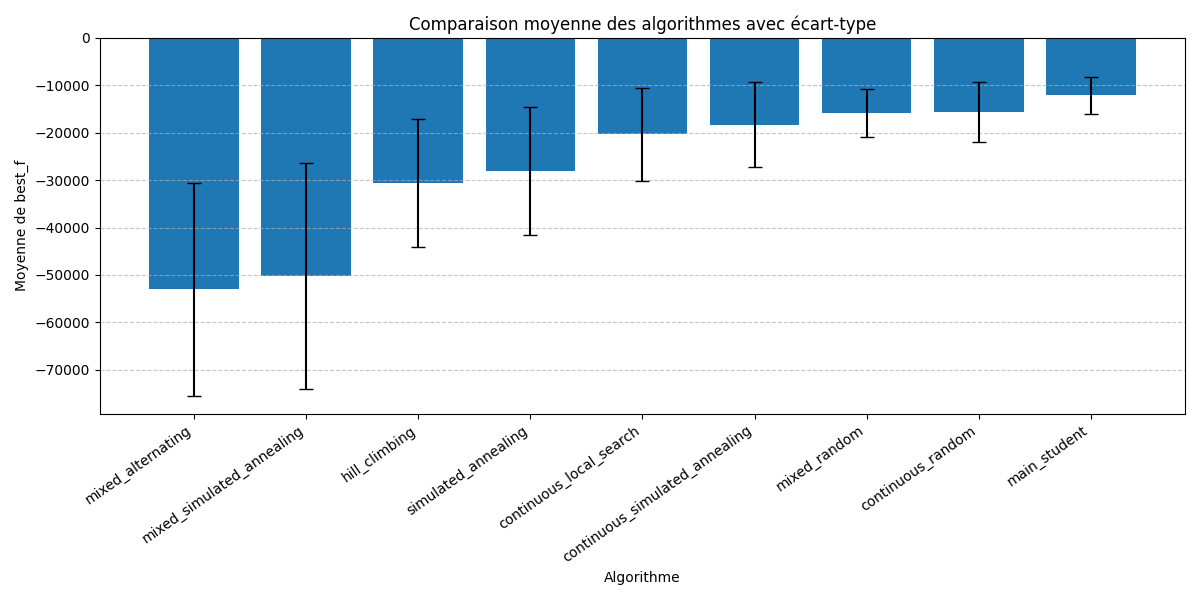
\includegraphics[width=\textwidth]{Comparaison_moyenne_algoNN.png}
    \caption{Comparaison moyenne des algorithmes avec écart-type}
    \label{fig:comparison}
\end{figure}

\subsection{Analyse}

Le graphique présente la moyenne de la meilleure fitness obtenue pour chaque algorithme, avec des barres d'erreur correspondant à l'écart-type sur les exécutions.

Les résultats montrent que les méthodes mixtes sont les plus performantes. 
L'algorithme \textbf{mixed\_alternating} obtient la meilleure moyenne, suivi de près par \textbf{mixed\_simulated\_annealing}. 
Cela confirme l'intérêt d'optimiser simultanément les variables binaires et continues du problème mixQUBO.

Les méthodes combinatoires seules, comme \textbf{hill\_climbing} et \textbf{simulated\_annealing}, obtiennent des résultats intermédiaires. 
Elles exploitent efficacement la structure binaire du problème, mais ignorent l'optimisation des variables continues, ce qui limite leur performance.

Les méthodes continues seules, comme \textbf{continuous\_random}, \textbf{continuous\_local\_search} et \textbf{continuous\_simulated\_annealing}, sont moins performantes. 
Cela indique que la partie binaire joue un rôle important dans la structure du problème.

Les méthodes aléatoires donnent également des résultats plus faibles, car elles n'exploitent pas suffisamment le voisinage des solutions.

Les écarts-types montrent une variabilité plus importante pour les méthodes mixtes. 
Cette variabilité est cohérente avec le fait que ces méthodes explorent un espace de recherche plus grand, combinant à la fois variables binaires et continues.

Ainsi, les résultats confirment que les approches hybrides sont les plus adaptées pour résoudre efficacement le problème mixQUBO.

\section{Conclusion}

Ce projet a permis de comparer plusieurs méthodes d'optimisation sur le problème mixQUBO.

Les résultats expérimentaux montrent clairement que les méthodes hybrides sont les plus efficaces. 
En particulier, \textbf{mixed\_alternating} obtient les meilleures performances moyennes, suivi de \textbf{mixed\_simulated\_annealing}.

Les méthodes purement combinatoires restent intéressantes, mais elles sont limitées par le fait que les variables continues ne sont pas optimisées. 
Inversement, les méthodes purement continues ne suffisent pas à capturer la structure principale du problème.

L'optimisation mixte apparaît donc comme l'approche la plus adaptée pour ce type de problème.

\subsection{Perspectives}

Plusieurs améliorations peuvent être envisagées :
\begin{itemize}
    \item ajuster automatiquement les paramètres des algorithmes
    \item améliorer le refroidissement du recuit simulé
    \item utiliser des voisinages plus riches
    \item combiner les méthodes avec des stratégies de restart plus avancées
    \item tester des métaheuristiques plus sophistiquées comme CMA-ES ou des méthodes hybrides adaptatives
\end{itemize}

\end{document}